\documentclass[11pt]{book}
\usepackage[colorlinks = true,linkcolor = blue]{hyperref}
\usepackage[letterpaper]{geometry} % Custom margins
\usepackage{graphicx}
\usepackage[spanish]{babel}
\usepackage[T1]{fontenc}
\usepackage[utf8]{inputenc}
\usepackage{remreset}

\makeatletter
  \@removefromreset{section}{chapter}
\makeatother
\addto\captionsspanish{\renewcommand{\chaptername}{}}
\renewcommand{\thechapter}{Unidad \arabic{chapter}}
\renewcommand{\thesection}{S\arabic{section}}
\renewcommand{\thesubsection}{L\arabic{subsection}}
\setlength{\parindent}{0pt}

\begin{document}
\pagestyle{empty}
\newgeometry{letterpaper,left=15mm,top=50mm,bottom=0mm} % Custom margins
\begin{center}
  {\Huge F\'isica}\\
  \vspace{2cm}
  \normalsize
  \textbf{\large Cuaderno de trabajo}\\
  para los alumnos de 2$^\circ$ de  Secundaria\\
  en el curso durante el ciclo escolar\\
  \textbf{2022-2023}\\
  \vspace{2.5cm}
  \small POR\\
  \Large J. C. Melchor Pinto\\[0.5em]
  \normalsize Profesor de asignatura en\\
  \vspace{1cm}
  
\includegraphics[width=4cm]{./Unidad 2/Images/LOGO_RDS_nobg}
\end{center}
\vspace{2cm}
%\include*{Functional/TitlePage}
\hspace{-16mm}
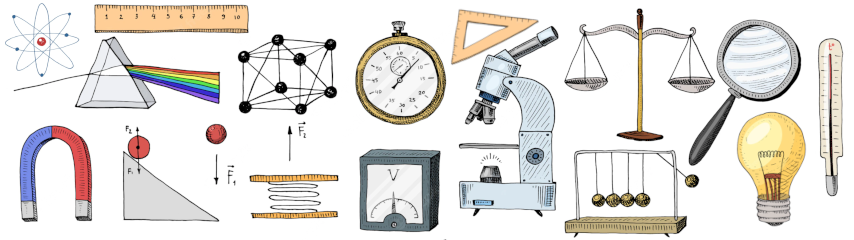
\includegraphics[width=\paperwidth]{./Unidad 2/Images/cover_bg}
\restoregeometry
\tableofcontents
\chapter{}

\section{Tecnología y transformación de la sociedad}
\subsection{El cambio y el tiempo}

\section{Velocidad y aceleración}
\subsection{El movimiento de los objetos}
\subsection{La velocidad y la rapidez}
\subsection{Gráficas que representan la velocidad (desplazamiento vs. tiempo)}
\subsection{La aceleración como cambio de la velocidad}

\section{Movimiento ondulatorio}
\subsection{Ondas para ''ver''}

\section{Concepto de fuerza}
\subsection{La fuerza como interacción entre los objetos}
\subsection{Suma de fuerzas}
\subsection{Máquinas simples}

\section{Leyes de Newton}
\subsection{Primera Ley de Newton}
\subsection{Segunda Ley de Newton}
\subsection{Tercera Ley de Newton}

\section{La aportación de Newton}
\subsection{Ley de Gravitación Universal}
\subsection{Newton, vida y obra, sus aportaciones para la ciencia}
\subsection{El movimiento regular de los cuerpos del Sistema Solar: las leyes de Kepler}


\chapter{}

\section{La energía y sus manifestaciones}
\subsection{Tipos de energía}
\subsection{La conservación de la energía mecánica}

\section{Los modelos en la ciencia}
\subsection{Explicación de los fenómenos de la naturaleza a partir de modelos}
\subsection{Ideas en la historia entorno a la estructura de la materia}
\subsection{Aspectos básicos del modelo cinético de partículas}

\section{Cambios de estado de la materia y el modelo cinético}
\subsection{Propiedades de la materia: forma, volumen, estados de agregación, compresibilidad, etcétera}
\subsection{Cambios de estado de agregación}

\section{Temperatura y equilibrio térmico}
\subsection{Temperatura}
\subsection{Calor y temperatura}

\section{Calor como energía}
\subsection{Energía térmica}
\subsection{Calor y otras formas de energía}
\subsection{Energía eléctrica y medio ambiente}

\section{Interacciones eléctricas}
\subsection{Fenómenos electrostáticos}

\section{El modelo atómico de la materia}
\subsection{Descripción macroscópica y microscópica del Universo}
\subsection{Desarrollo histórico del modelo atómico}
\subsection{Características del átomo}


\chapter{}

\section{Corriente eléctrica y magnetismo}
\subsection{Corriente eléctrica y magnetismo}
\subsection{Electromagnetismo}

\section{Electricidad y magnetismo: ondas electromagnéticas}
\subsection{Relación entre electricidad y magnetismo}
\subsection{Inducción electromagnética}
\subsection{Generación de ondas electromagnéticas}
\subsection{La luz visible}

\section{Electricidad y temperatura en sistemas biológicos}
\subsection{La física del cuerpo humano}

\section{Ciencia, tecnología y sociedad}
\subsection{Ciencia y tecnología aplicada a la salud}
\subsection{Ciencia y tecnología en el mundo actual}

\section{Física y conocimiento del Universo}
\subsection{La estructura del Universo}
\subsection{¿Cómo se estudia el Universo?}
\subsection{Los mecanismos de las estrellas}

\section{El Sistema Solar}
\subsection{Características y exploración del Sistema Solar}
\subsection{Origen del Sistema Solar}

\section{Origen y evolución del Universo}
\subsection{Teoría de la Gran Explosión}




\end{document}






